\documentclass{article}
% if you need to pass options to natbib, use, e.g.:
%     \PassOptionsToPackage{numbers, compress}{natbib}
% before loading neurips_2023
\usepackage[final]{neurips}
% to avoid loading the natbib package, add option nonatbib:
%    \usepackage[nonatbib]{neurips}


\usepackage[utf8]{inputenc} % allow utf-8 input
\usepackage[T1]{fontenc}    % use 8-bit T1 fonts
\usepackage{hyperref}       % hyperlinks
\usepackage{url}            % simple URL typesetting
\usepackage{booktabs}       % professional-quality tables
\usepackage{amsmath}        % math environments and \text{}
\usepackage{amsfonts}       % blackboard math symbols
\usepackage{nicefrac}       % compact symbols for 1/2, etc.
\usepackage{microtype}      % microtypography
\usepackage{xcolor}         % colors
\usepackage{graphicx}       % figures
\usepackage{array}          % extended table column specs
\usepackage{float}          % [H] placement for figures


\title{ML Application in Smart Grids --- Multi-class Intrusion Detection in Substation Traffic}


\author{%
  Hengyu Liu\\
  Department of ECE\\
  University of Toronto\\
  \texttt{hengyu.liu@mail.utoronto.ca} \\
  \And
  Jake Shi\\
  Department of ECE\\
  University of Toronto\\
  \texttt{jake.shi@utoronto.ca} \\
  \And
  Jiakai Tang\\
  Department of ECE\\
  University of Toronto\\
  \texttt{jiakai.tang@mail.utoronto.ca} \\
}

\begin{document}


\maketitle


\begin{abstract}
Modern electrical substations utilizing IEC104 over TCP/IP require robust intrusion detection systems to defend against sophisticated cyber-physical threats. This work develops a multi-class ML framework that classifies benign traffic and identifies specific attack vectors---denial-of-service, flooding, fuzzing, and replay attacks---using protocol-aware features extracted from IEC104 TCP/IP flows. SVM and FNN classifiers are evaluated via stratified validation with explicit class-imbalance mitigation, and assessed using macro-averaged F1-scores and confusion matrix analysis. Results demonstrate the efficacy of protocol-aware machine learning in enhancing the security posture of critical electrical infrastructure.
\end{abstract}

\section*{Attestation of Teamwork}
\textbf{Hengyu Liu} implemented the Feedforward Neural Network (FNN) model, including architecture design, hyperparameter selection, and training loop.

\textbf{Jake Shi} implemented the three-phase SVM pipeline --- baseline, improved, and optimised --- including feature selection via ANOVA F-test, hyperparameter optimisation via GridSearchCV, and multi-seed robustness evaluation.

\textbf{Jiakai Tang} coordinated the overall project, managed the shared GitHub repository, and led the dataset sourcing and data pre-treatment pipeline --- designing and implementing the class-specific resampling strategy.


\section{Introduction}

Modern power grids rely on the IEC 60870-5-104 (IEC 104) standard for SCADA communication. While this TCP/IP integration improves operational efficiency, it substantially expands the attack surface of critical infrastructure, as demonstrated by the 2015 Ukraine power grid compromise. Current intrusion detection systems (IDS) depend largely on static, signature-based rules. These inevitably lag behind emerging threats, struggling to identify novel or protocol-specific attacks without continuous manual updates.

Machine learning (ML) offers an adaptive alternative by learning discriminative patterns directly from network flows. This project evaluates two ML classifiers---a Support Vector Machine (SVM) and a Feedforward Neural Network (FNN)---for multi-class intrusion detection on IEC 104 traffic. Utilizing a public dataset of approximately 320,000 flows, we address key challenges including severe class imbalance (95.2\% DoS traffic) and high-dimensional feature spaces (84 dimensions).


\section{Preliminaries and Problem Formulation}

\textbf{IEC 104 Protocol.} The IEC 60870-5-104 standard enables remote monitoring and control between field devices and control centers in electrical substations. By adopting standard internet transport layers (TCP/IP), it inherits vulnerabilities to conventional network-layer attacks, including DoS flooding and session interception.

\textbf{Network Flow Features.} We utilize CICFlowMeter to extract 84-dimensional feature vectors from raw packet captures. These protocol-agnostic features capture the statistical properties of bidirectional communication sessions (e.g., packet inter-arrival times, TCP flag counts), effectively encoding behavioral signatures suitable for ML classifiers.

\textbf{Dataset.} This project uses a public Zenodo dataset~[1] comprising 319,971 network flows and described in detail in the accompanying Data in Brief publication~[2]. Crucially, the normal traffic reflects authentic IEC 104 communication captured from an operational Ukrainian substation. The seven attack categories (DoS, flood, fuzzy, MITM, IEC-104 starvation, NTP DDoS, and port scan) were safely generated in a replicated laboratory testbed.

\section{Design}

\subsection{SVM-Based Intrusion Detection}

We design an SVM-based classifier for IEC 104 SCADA network intrusion detection that distinguishes normal traffic from six attack types (flood, fuzzy, MITM, IEC-104 starvation, NTP DDoS, and port scan). The system follows a three-phase improvement pipeline:

\textbf{Phase 1 (Baseline)} uses a linear-kernel SVM with default parameters on raw, unscaled features. This establishes a performance floor by deliberately omitting scaling, non-linear kernels, and class balancing.

\textbf{Phase 2 (Improved)} addresses each baseline weakness: StandardScaler normalises features to zero-mean unit-variance, ANOVA F-test selects the 30 most discriminative features, an RBF kernel captures non-linear decision boundaries, and \texttt{class\_weight='balanced'} up-weights minority classes inversely proportional to their frequency.

\textbf{Phase 3 (Optimised)} performs exhaustive hyperparameter tuning via GridSearchCV over $C \in \{0.1, 1, 10, 100\}$, $\gamma \in \{\text{scale}, \text{auto}, 0.01, 0.1\}$, and $\text{kernel} \in \{\text{rbf}, \text{poly}\}$, evaluated with 5-fold stratified cross-validation scored by weighted-F1.

\subsection{Feedforward Neural Network (FNN)}

A complementary FNN classifier uses fully connected layers with ReLU activations, a softmax output layer, cross-entropy loss, and the Adam optimiser.

\section{Methodology}

\subsection{Data Over/Under Sampling Methodology}

The raw dataset is severely imbalanced: \texttt{dosattack} dominates with 304,627 flows (95.2\%) while \texttt{mitmattack} holds only 26 flows (ratio 11,716:1). Training on this distribution collapses classifiers to majority-class prediction, yielding misleadingly high accuracy but near-zero macro-F1. A class-specific resampling strategy (Table~\ref{tab:resampling}) was applied to the training fold after the stratified split.

\begin{table}[ht]
  \caption{Class-specific resampling strategy applied to the IEC 104 dataset.}
  \label{tab:resampling}
  \centering
  \setlength{\tabcolsep}{4pt}
  \footnotesize
  \begin{tabular}{lrrp{2.3cm}p{5.0cm}}
    \toprule
    \textbf{Label} & \textbf{Original} & \textbf{Target} & \textbf{Treatment} & \textbf{Rationale} \\
    \midrule
    \texttt{dosattack}        & 304,627 & $\sim$10,000   & Random Undersample  & Preserves DoS patterns while removing massive bias; 10k is sufficient for the model to learn. \\
    \texttt{portscanattack}   & 9,710   & $\sim$5,000    & ClusterCentroids    & Reduces redundancy in dense majority regions while keeping a strong decision boundary. \\
    \texttt{ntpddosattack}    & 2,278   & $\sim$3,000    & SMOTE               & Slight oversampling groups it with mid-tier classes for more balanced training. \\
    \texttt{iec104starvation} & 2,028   & $\sim$3,000    & SMOTE               & Slight oversampling to match NTP DDoS tier and equalise representation. \\
    \texttt{attackfree}       & 255     & $\sim$3,000    & SMOTE / SMOTENC     & Aggressive oversampling needed; maximising normal-class coverage minimises false positives. \\
    \texttt{fuzzyattack}      & 939     & $\sim$2,000    & ADASYN              & Adaptive synthesis focuses on harder boundaries typical of randomised fuzzy payloads. \\
    \texttt{floodattack}      & 108     & $\sim$1,000    & SMOTE               & A $\sim$10$\times$ synthetic boost approaches the safe upper limit before SMOTE quality degrades. \\
    \texttt{mitmattack}       & 26      & $\sim$250--500 & Random Oversample   & Pure duplication (10--20$\times$) keeps the class recognisable without introducing synthetic artefacts. \\
    \bottomrule
  \end{tabular}
\end{table}

SMOTE and ADASYN were applied only to the training fold to prevent data leakage; the test set retains the original class distribution.

\subsection{SVM Methodology}

\textbf{Data Preprocessing.} The dataset comprises 7 CSV files from CICFlowMeter containing 84 columns per flow. We drop four metadata columns (Flow ID, Src/Dst IP, Timestamp), replace infinite values and NaNs with column medians, and encode the target label via LabelEncoder. A 75/25 stratified train-test split preserves class proportions.

\textbf{Feature Selection.} ANOVA F-test ranks features by their between-class to within-class variance ratio. We retain the top 30 features; the highest-scoring features (SYN Flag Count, Fwd PSH Flags, FIN Flag Count) align with known IEC 104 attack signatures.

\textbf{Multi-Seed Evaluation.} We run the full three-phase pipeline with five different random seeds ($\{42, 123, 256, 789, 1024\}$) and report the averaged metrics with standard deviations.

\textbf{Implementation.} Python using scikit-learn (SVC, GridSearchCV, StandardScaler, SelectKBest), pandas, and matplotlib/seaborn.

\subsection{FNN Methodology}

\textbf{Data Preprocessing.} Non-numeric and irrelevant features (Flow ID, IP addresses, timestamps, ports) were removed. Remaining features were converted to numeric format, missing values filled with zeros, and samples with missing labels removed.

\textbf{Data Splitting.} 80/20 stratified split preserving class proportions.

\textbf{Dataset Balancing.} The class-specific resampling strategy from Section~4.1 was applied to the training fold.

\textbf{Training.} The FNN was trained for 20 epochs using the Adam optimiser with cross-entropy loss.

\section{Numerical Experiments}

\subsection{SVM Results}

Table~\ref{tab:svm-results} presents the averaged performance metrics across five random seeds for each improvement phase.

\begin{table}[ht]
  \caption{SVM performance across improvement phases (mean $\pm$ std over 5 seeds).}
  \label{tab:svm-results}
  \centering
  \begin{tabular}{lccc}
    \toprule
    \textbf{Metric} & \textbf{Phase 1 (Baseline)} & \textbf{Phase 2 (Improved)} & \textbf{Phase 3 (Optimised)} \\
    \midrule
    Accuracy         & $0.964 \pm 0.002$ & $0.999 \pm 0.000$ & $\mathbf{1.000 \pm 0.000}$ \\
    F1 (weighted)    & $0.957 \pm 0.003$ & $0.999 \pm 0.000$ & $\mathbf{1.000 \pm 0.000}$ \\
    F1 (macro)       & $0.449 \pm 0.022$ & $0.894 \pm 0.015$ & $\mathbf{0.933 \pm 0.010}$ \\
    Precision (wt)   & $0.959 \pm 0.003$ & $1.000 \pm 0.000$ & $\mathbf{1.000 \pm 0.000}$ \\
    Recall (wt)      & $0.964 \pm 0.002$ & $0.999 \pm 0.000$ & $\mathbf{1.000 \pm 0.000}$ \\
    \bottomrule
  \end{tabular}
\end{table}

The baseline achieves 96.4\% accuracy but only 44.9\% macro-F1, indicating failure on minority classes. Phase 2 lifts macro-F1 from 0.449 to 0.894. Phase 3's GridSearchCV reaches 93.3\% macro-F1, selecting a polynomial kernel with $C=100$ and $\gamma=0.1$.

\begin{figure}[ht]
  \centering
  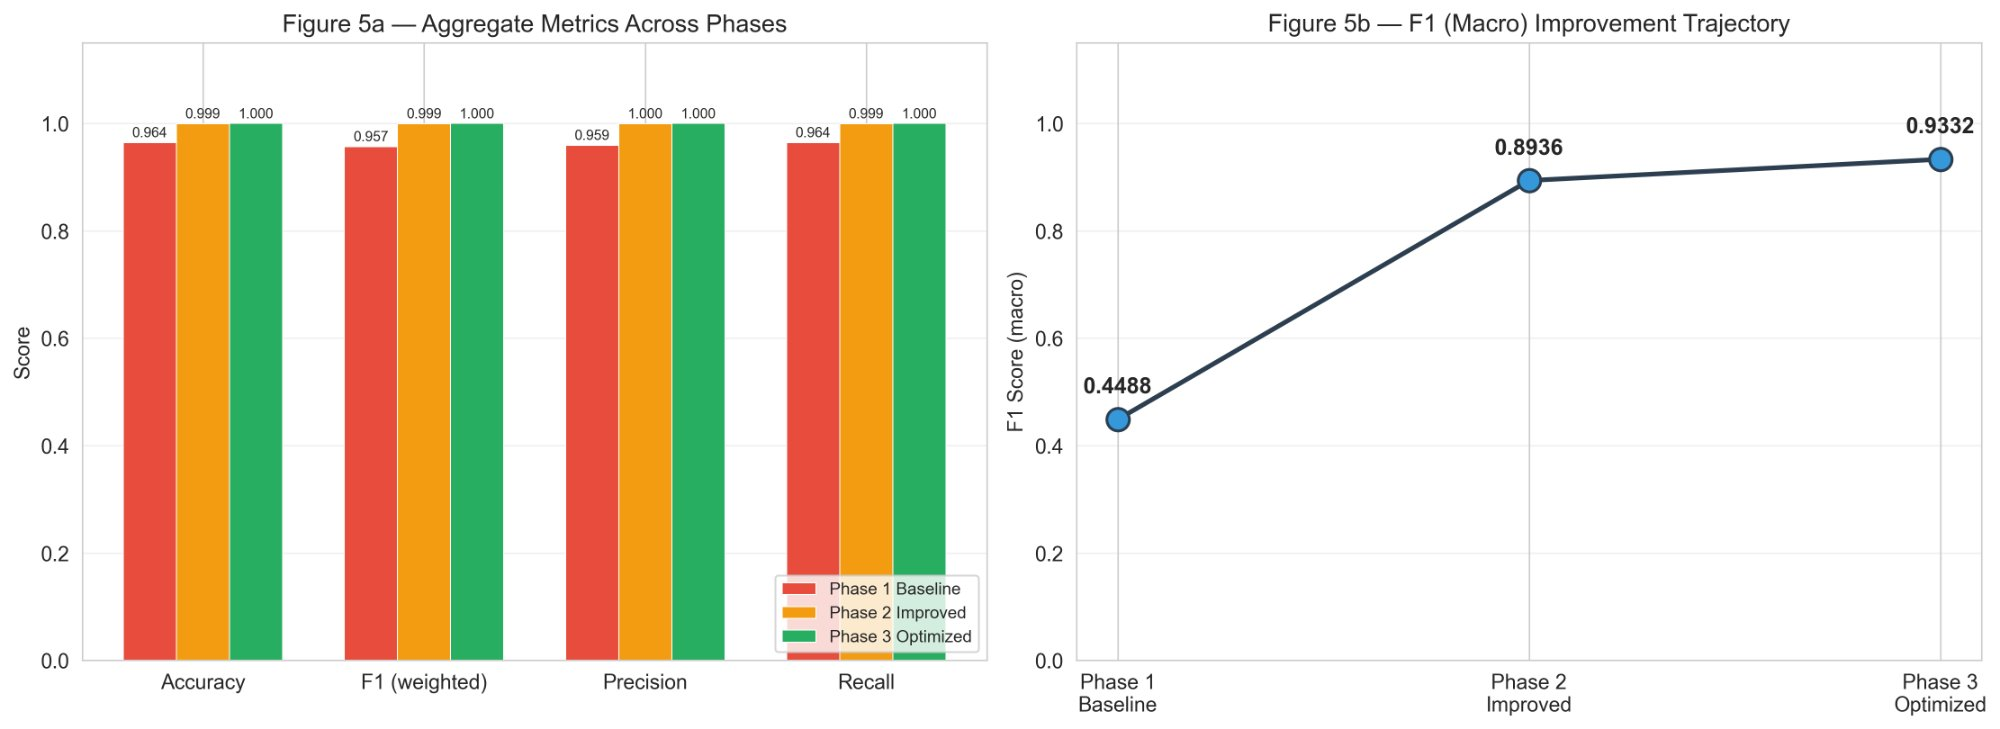
\includegraphics[width=0.92\textwidth]{figures/image1.png}
  \caption{SVM performance metrics across phases (left) and F1 macro trajectory (right).}
  \label{fig:svm-phases}
\end{figure}

\begin{figure}[ht]
  \centering
  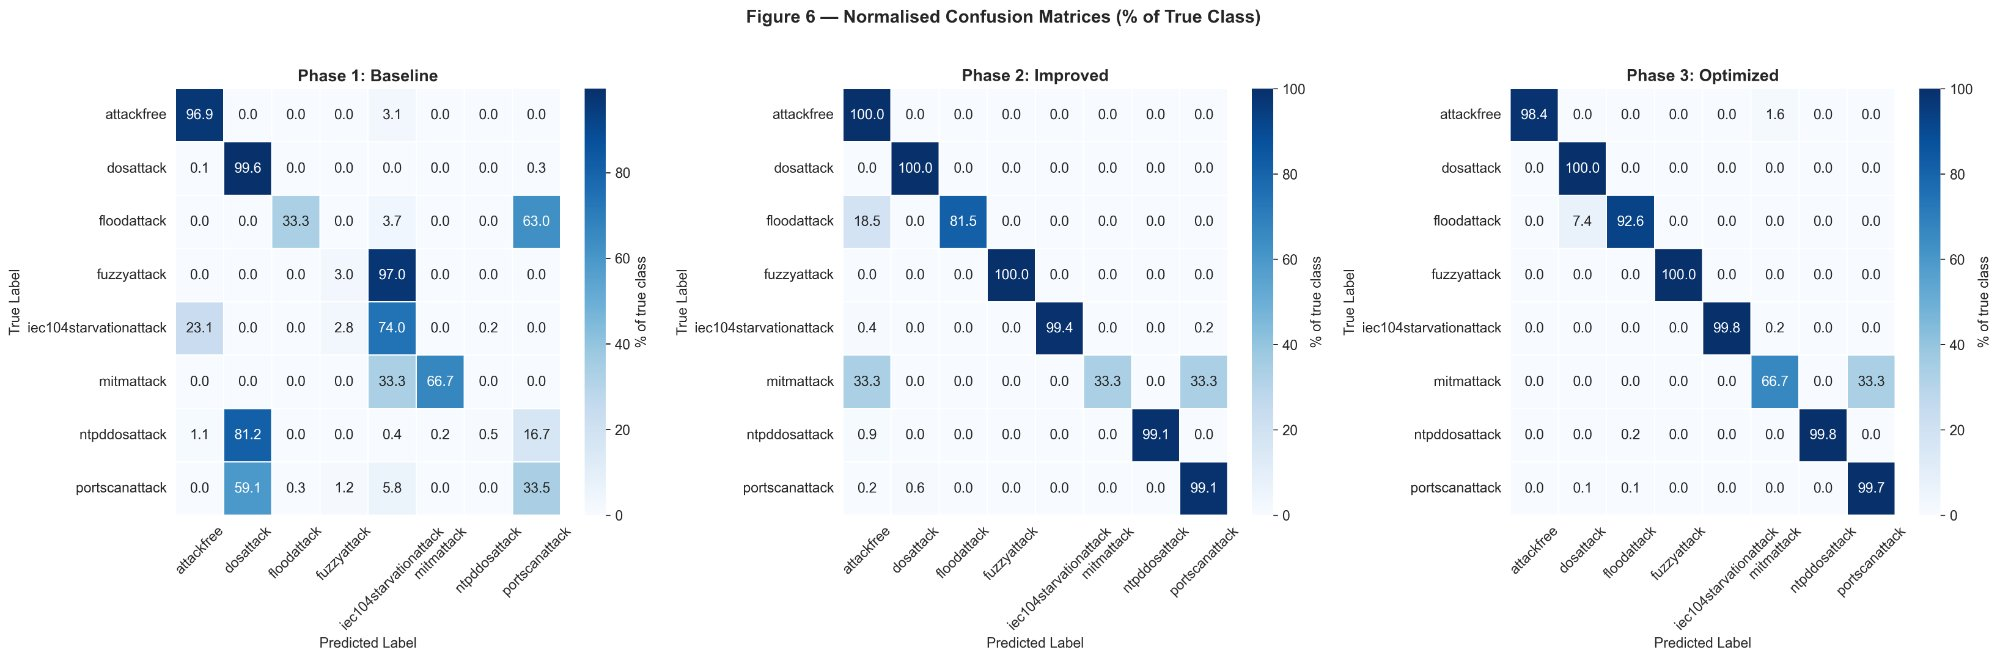
\includegraphics[width=\textwidth]{figures/image2.png}
  \caption{Normalised confusion matrices (\% of true class) for each SVM phase.}
  \label{fig:svm-confusion}
\end{figure}

\subsection{FNN Results}

The FNN was trained for 20 epochs. On the original imbalanced dataset, validation accuracy reached 100\% almost immediately. After applying dataset balancing through resampling, the model exhibited a more reasonable convergence, with validation accuracy stabilising at approximately 99.6\%.

\begin{figure}[ht]
  \centering
  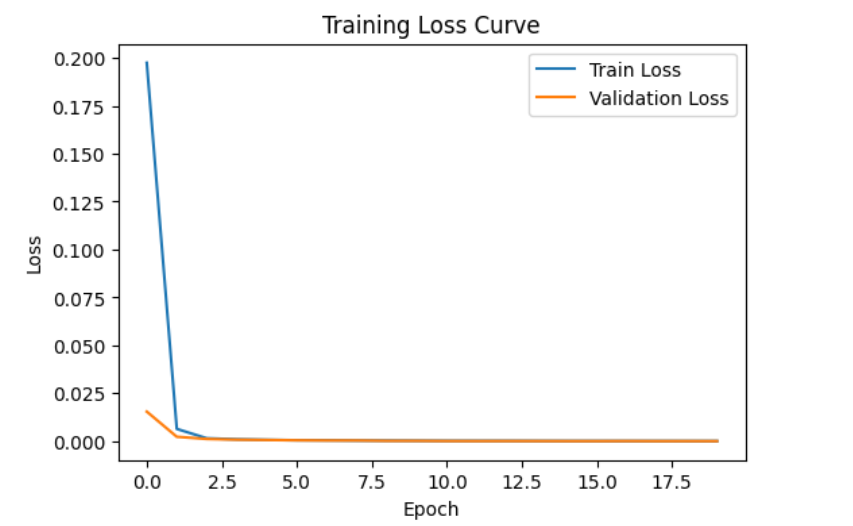
\includegraphics[width=0.55\textwidth]{figures/image3.png}
  \caption{FNN training loss and validation accuracy over 20 epochs.}
  \label{fig:fnn-training}
\end{figure}


\section{Discussion}

\subsection{SVM Analysis}

\textbf{Impact of preprocessing.} The dominant improvement comes from Phase 2, not Phase 3. Feature scaling is critical for SVMs because the RBF kernel's distance computation is dominated by high-range features without normalisation. Class balancing was equally important --- without it, the SVM ignores classes with fewer than 100 samples.

\textbf{Remaining challenges.} MITM detection remains the weakest point ($\text{F1} \approx 0.57$--$0.67$), attributable to its small sample size (26 flows). Data augmentation could further improve minority-class performance.

\textbf{Multi-seed robustness.} Low standard deviations ($\leq 0.022$) confirm results are not artefacts of a single fortunate split.

\subsection{FNN Analysis}

\textbf{Effect of dataset balancing.} Resampling shifted the FNN from a spurious near-100\% accuracy (masking minority-class failure) to a meaningful 99.6\% with balanced learning across all classes.

\textbf{Data leakage concerns.} The extremely high accuracy on both models suggests features are highly informative, but may also indicate the lab-simulated dataset is relatively simple. Further validation on unseen operational data is necessary.

\subsection{Model Comparison}

Both classifiers achieved near-perfect accuracy. The SVM's three-phase pipeline illustrates the cumulative impact of preprocessing and tuning, while the FNN's rapid convergence reflects the dataset's high separability.

\section{Conclusions}

Both SVM and FNN classifiers, paired with appropriate preprocessing and class balancing, achieved near-perfect accuracy for multi-class IEC 104 intrusion detection. Two conclusions follow.

\textbf{Model Selection and Interpretability.} While both evaluated models perform well, Random Forest is more widely adopted in practice for SCADA IDS, offering high accuracy, better interpretability, and faster training on constrained resources~[3]. Interpretability is particularly important in critical infrastructure, where operators must understand and trust model decisions before acting on alerts.

\textbf{Transition to Production Readiness.} The current high accuracy is largely attributed to training on lab-simulated substation data --- a necessary step given the sensitivity and limited access to live power grid environments. While the attack-free data originates from a real Ukrainian substation~[2], the attack traffic was generated in a controlled testbed. It is critical to recognise that a retraining phase will be required with actual operational data to ensure the model's continued robustness and production readiness. Adversarial conditions in live grids may introduce traffic patterns not represented in the current dataset.


\newpage
\section*{References}
\medskip
{
\small

[1] IEC 104 SCADA Network Intrusion Detection Dataset, Zenodo, 2024. Available: \url{https://zenodo.org/records/15487636}

[2] B. Kuzlu et al., “IEC 104 SCADA network intrusion detection dataset,” {\it Data in Brief}, Elsevier, 2024. Available: \url{https://www.sciencedirect.com/science/article/pii/S2352340924011156}

[3] E. Michael, “Deep learning vs. traditional machine learning for intrusion detection in network security,” ResearchGate, Aug. 2024.
}

\clearpage
\section*{Appendix}

\subsection*{A. SVM Supplementary Figures}

\begin{figure}[H]
  \centering
  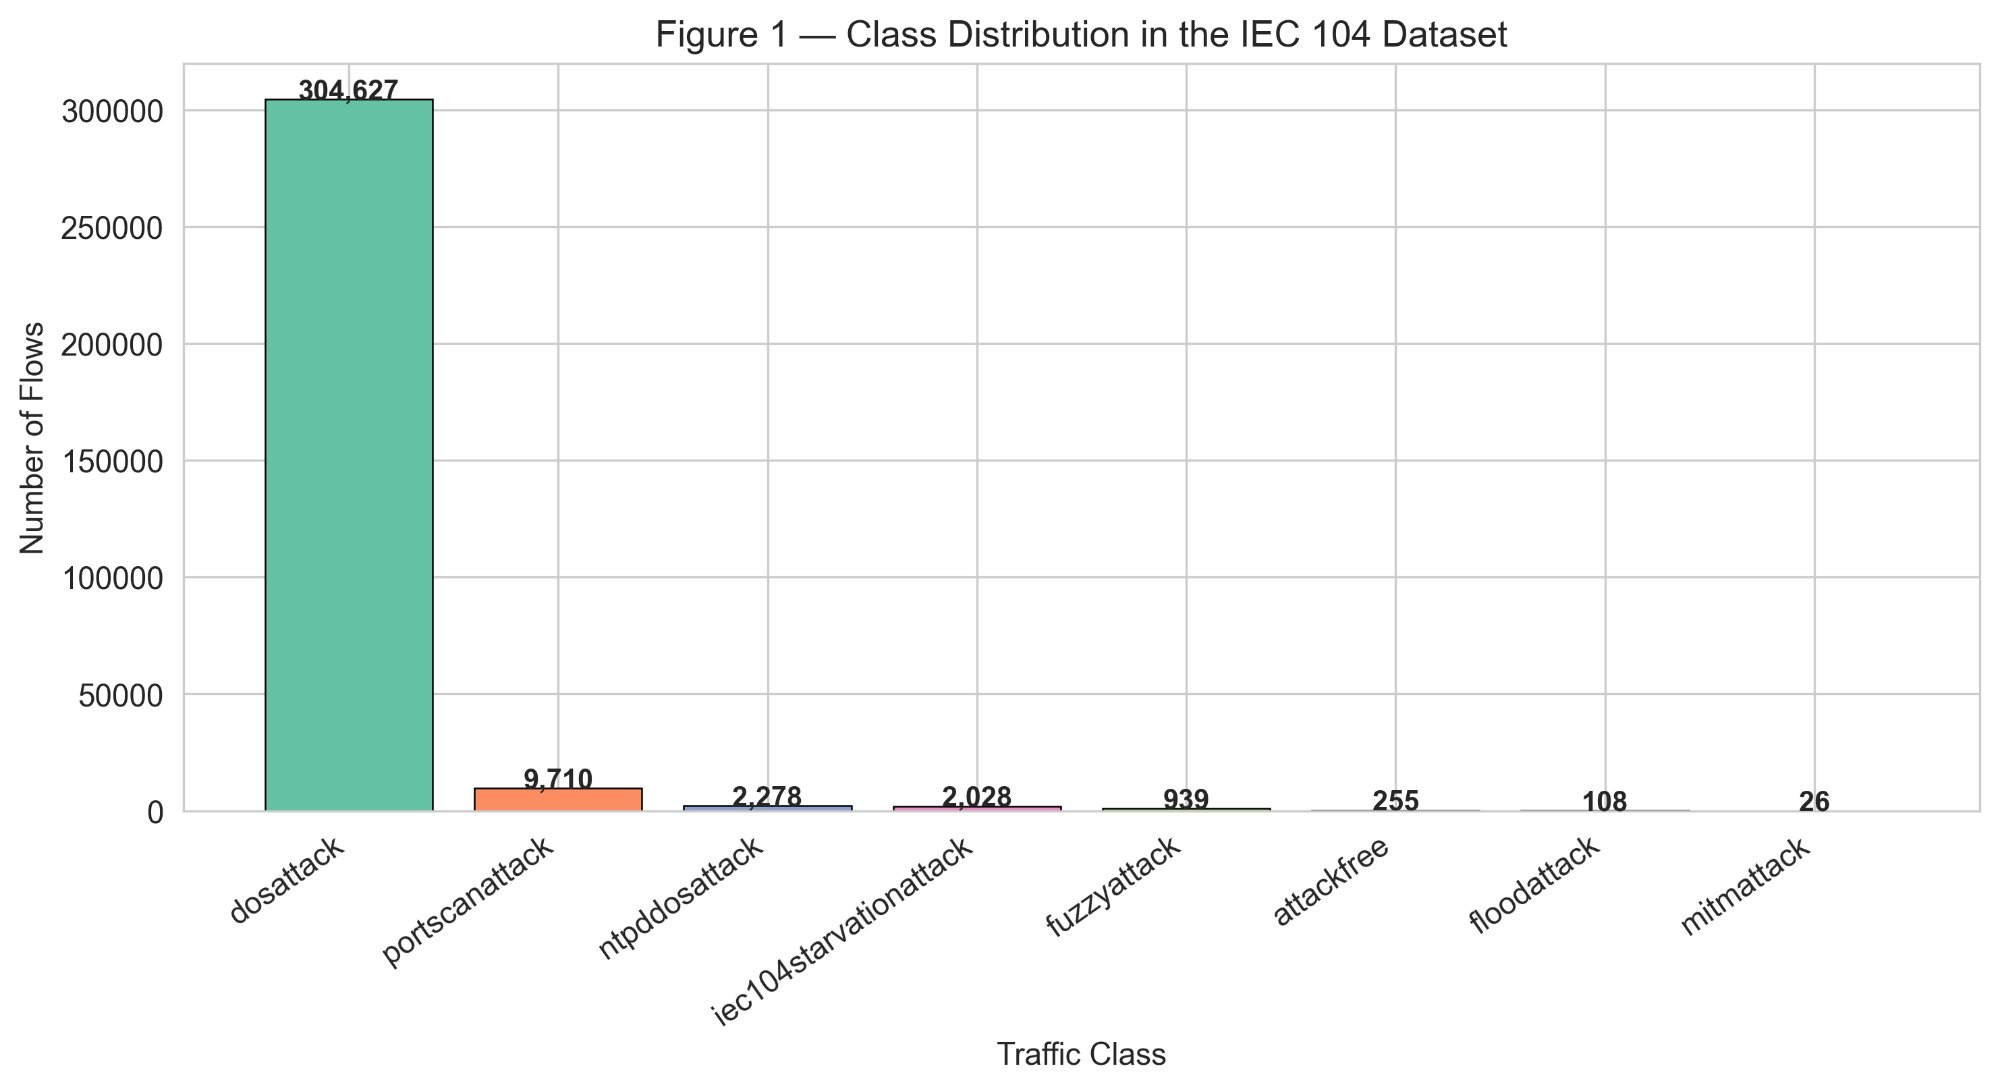
\includegraphics[width=0.88\textwidth]{figures/image4.png}
  \caption{Class distribution in the IEC 104 dataset.}
  \label{fig:class-dist}
\end{figure}

\begin{figure}[H]
  \centering
  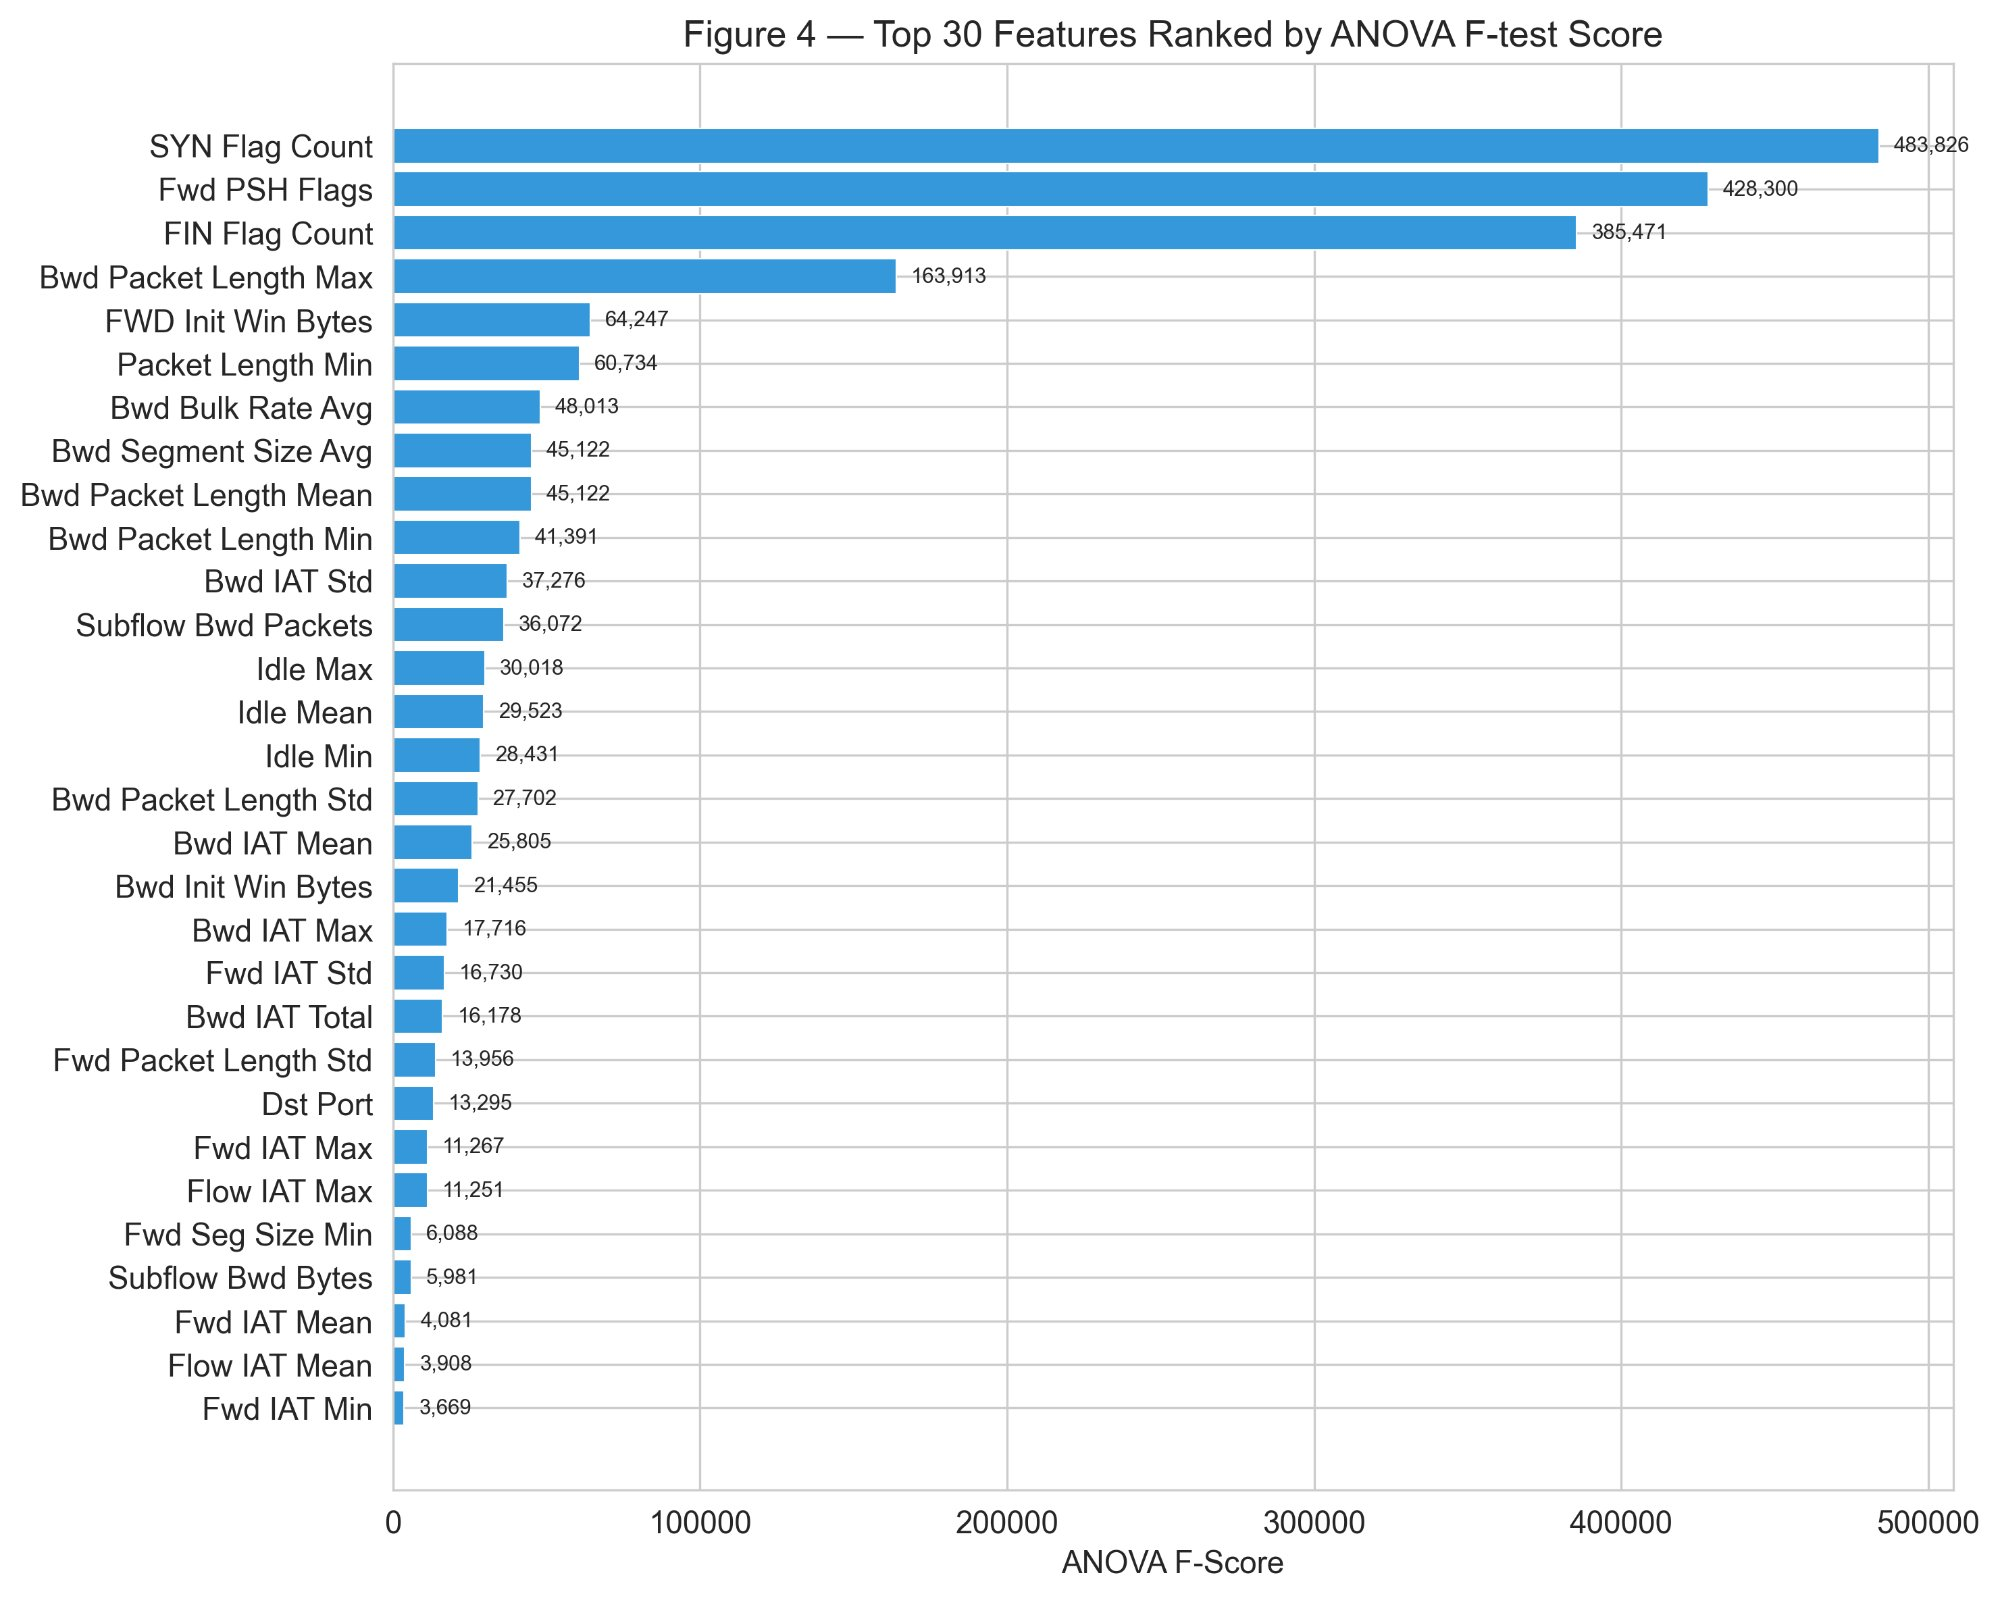
\includegraphics[width=0.85\textwidth]{figures/image5.png}
  \caption{Top 30 features ranked by ANOVA F-test score.}
  \label{fig:anova}
\end{figure}

\begin{figure}[H]
  \centering
  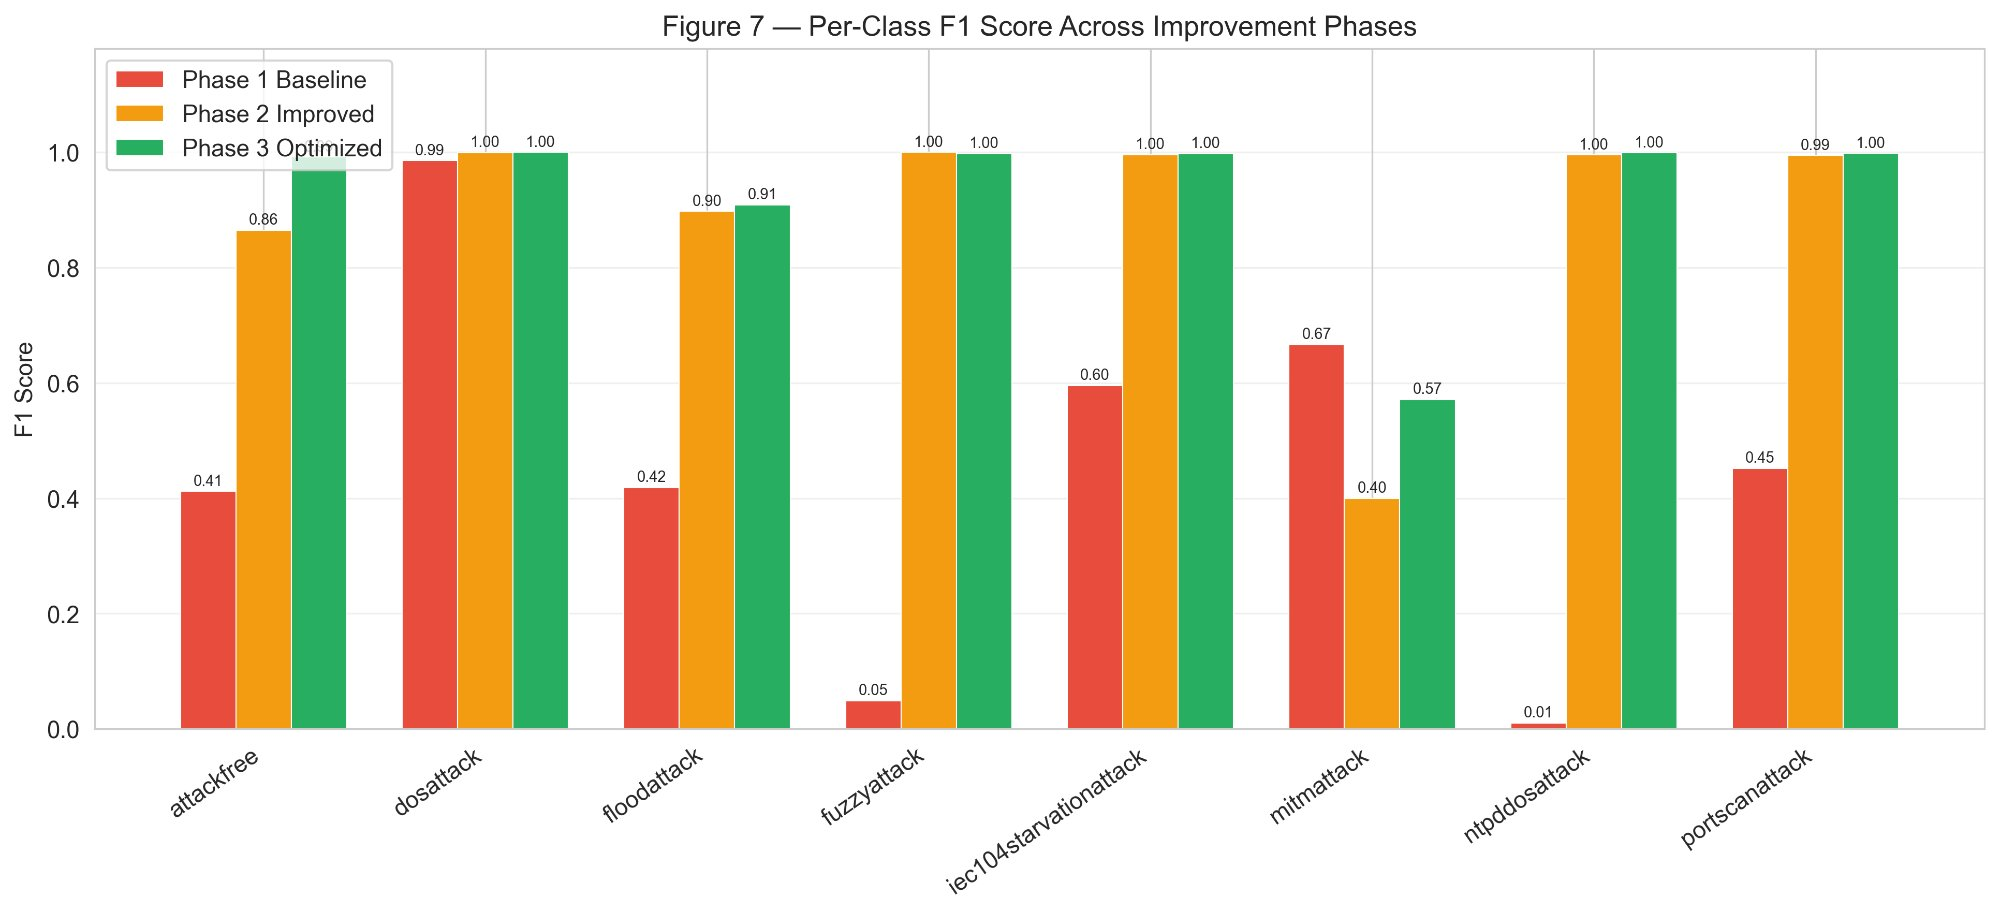
\includegraphics[width=0.92\textwidth]{figures/image6.png}
  \caption{Per-class F1 score across improvement phases.}
  \label{fig:perclass-f1}
\end{figure}

\begin{figure}[H]
  \centering
  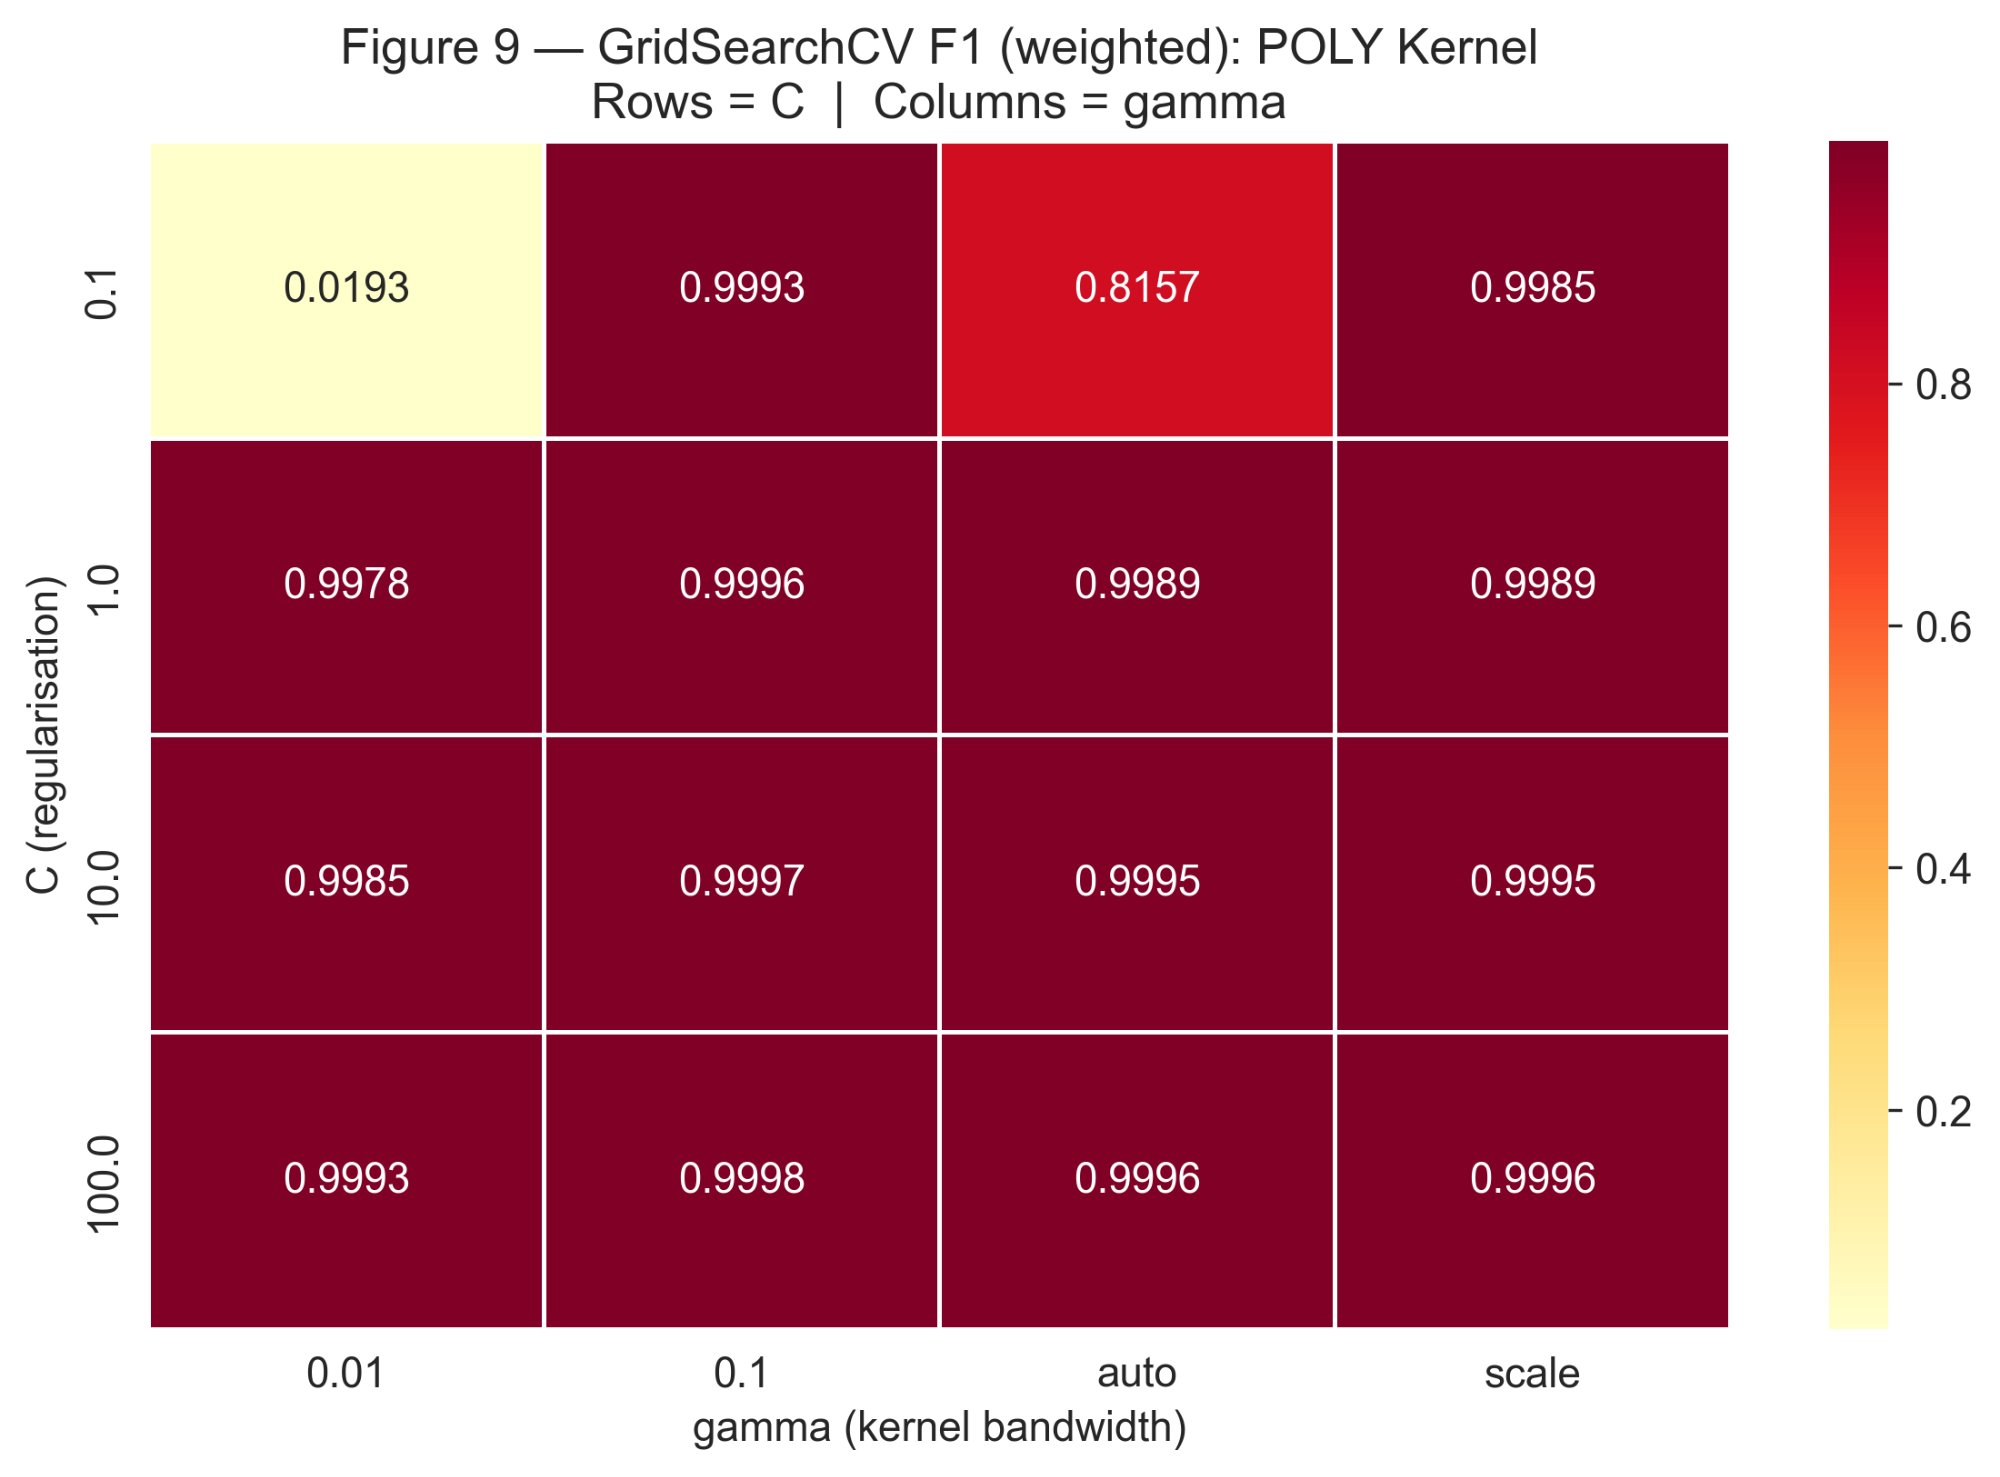
\includegraphics[width=0.70\textwidth]{figures/image7.png}
  \caption{GridSearchCV heatmap for the polynomial kernel.}
  \label{fig:gridsearch}
\end{figure}

\begin{figure}[H]
  \centering
  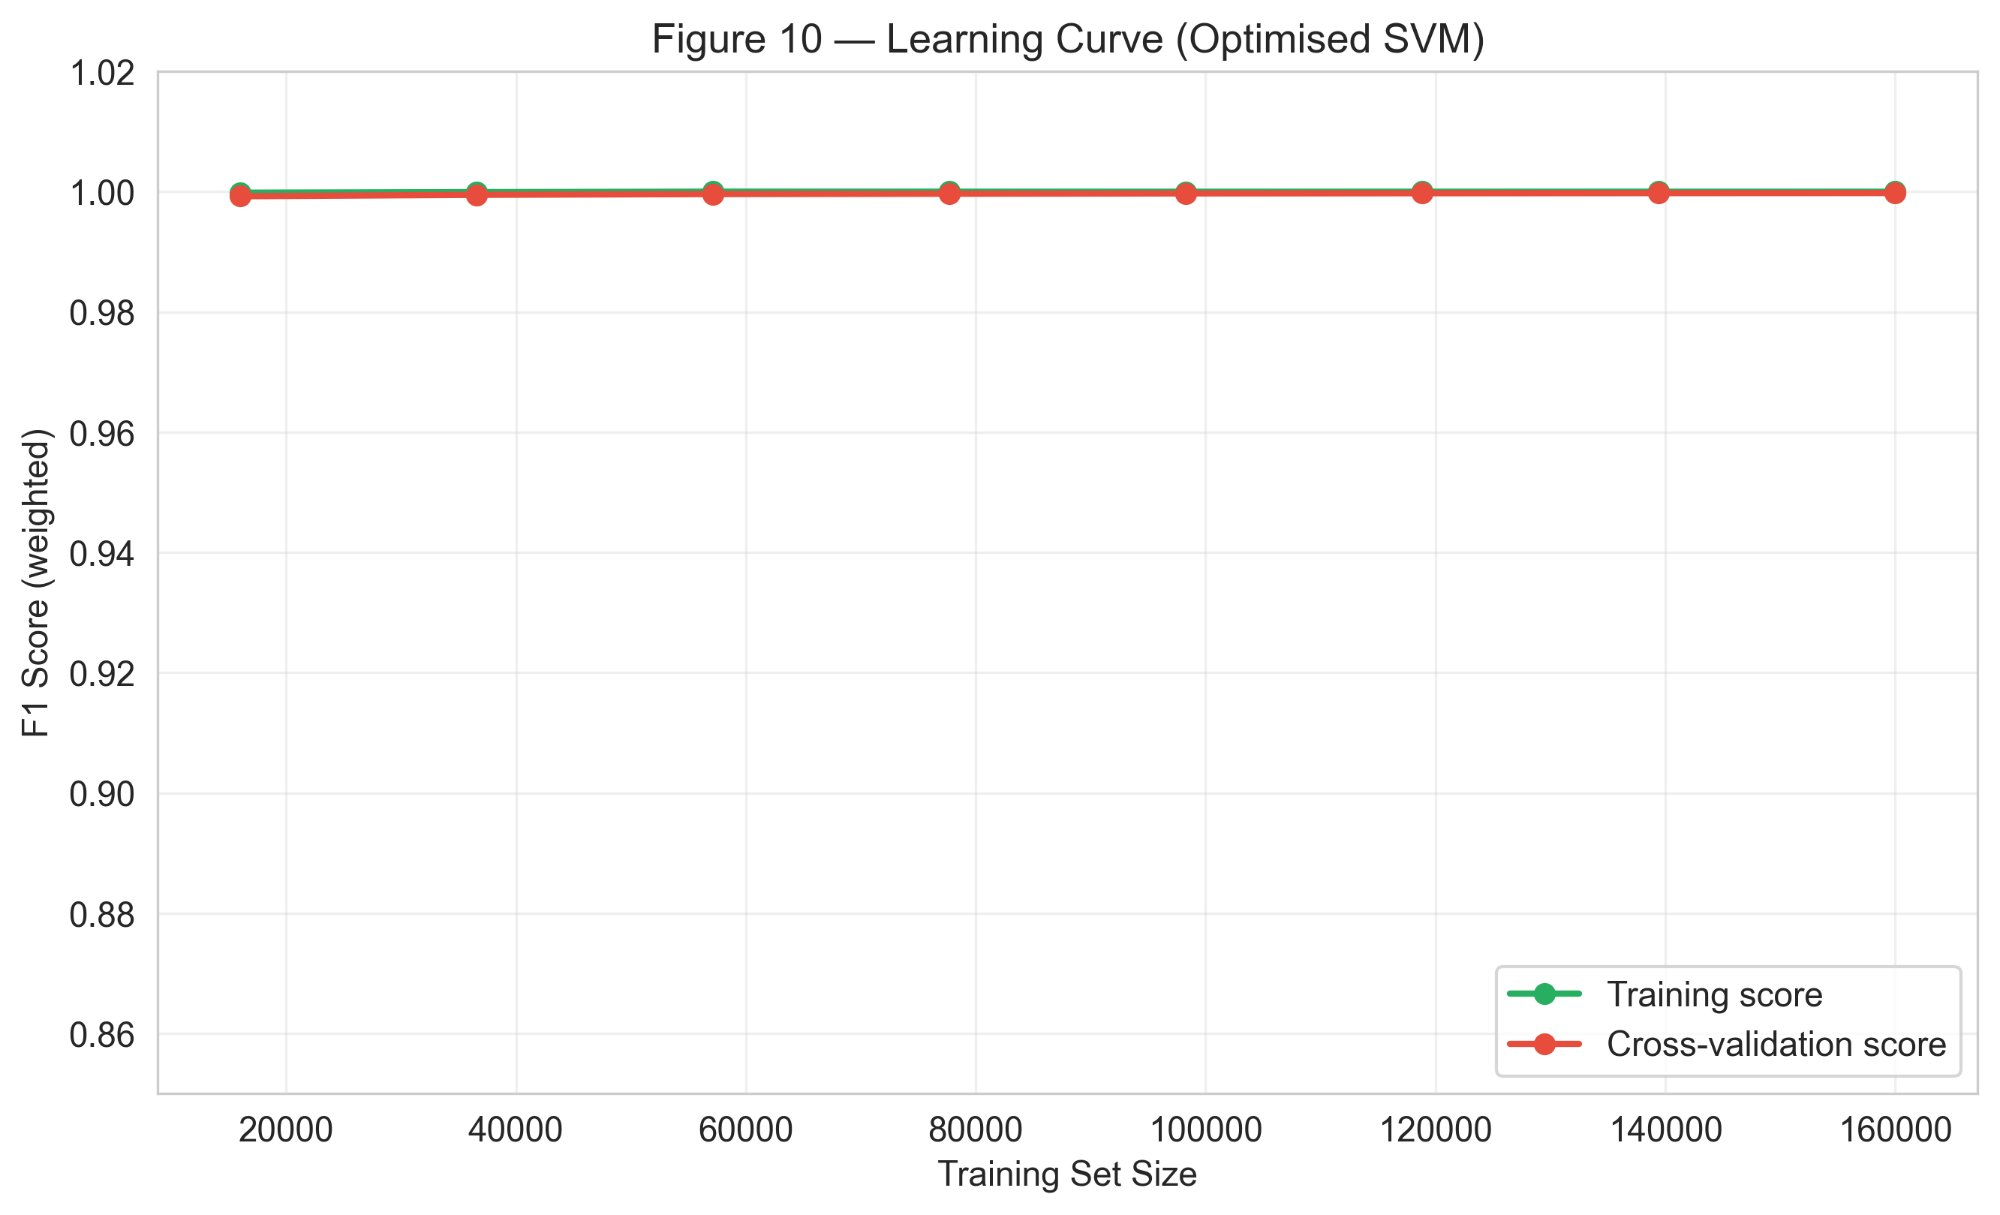
\includegraphics[width=0.72\textwidth]{figures/image8.png}
  \caption{Learning curve for the optimised SVM.}
  \label{fig:learning-curve}
\end{figure}

\clearpage
\section*{AI Usage}
Throughout this project, AI tools (e.g., Gemini) were used as a code explainer for the researched code. They were also used to help structure and refine written portions of the report. All technical decisions --- including model architecture, hyperparameter choices, resampling strategies, and experimental design --- were made independently by the group members. AI served as a productivity tool rather than a decision-maker, and all outputs were critically reviewed and validated by the team.

\section*{Contest for Information Sharing}
As part of this course, we may share selected project materials (e.g., reports, presentation slides, and presentation recordings) on the course webpage as learning resources for future students. Additionally, we may use anonymized project information for internal statistical analysis of course outcomes. Please indicate your preferences below. \textit{Your choices will not affect your grade in any way.}

\subsection*{Consent for Sharing Project Materials}
\textit{Please keep the item you wish and remove the other one.}

\begin{itemize}
	\item All group members consent to allow the project materials (report, slides, and presentation recording) to be shared on the course page for future students.
\end{itemize}

\subsection*{Consent for Use of Project Information in Statistical Analysis}
\textit{Please keep the item you wish and remove the other one.}
\begin{itemize}
	\item All group members consent to allow anonymized information about the project (e.g., topic, methods, outcomes, grades) to be used by the instructor for statistical analysis and course improvement.
\end{itemize}

\subsection*{Optional Comments}
\textit{Please list any specific conditions or comments here.}

\subsection*{Group Identification}

\begin{itemize}
	\item Group number: Group 10
	\item Names of group members: Hengyu Liu, Jake Shi, Jiakai Tang
	\item Signature of group members: Hengyu Liu, Jake Shi, Jiakai Tang
	\item Date: April 12, 2026
\end{itemize}

\end{document}
